% ------------------------------------------------------------------
% ------------------------------------------------------------------
% Demonstração de uso da classe ppgee.cls v1.1
% Autoria: Gabriel Gutierrez P. Soares <https://github.com/gutierrezps>
% 
% Modelo para elaboração de Dissertações e Teses do Programa de
% Pós-Graduação em Engenharia Elétrica do Instituto Federal da
% Paraíba (PPGEE-IFPB), Campus João Pessoa.
%
% Modelo elaborado de acordo com formatação do arquivo DOCX
% disponibilizado na página do PPGEE:
% https://www.ifpb.edu.br/ppgee/documentos/modelo-de-dissertacao/modelo_dissertacao_ppgee.docx
%
% PPGEE - IFPB: https://www.ifpb.edu.br/ppgee/
%
% Utilizando a classe abntex2 como base: https://www.abntex.net.br/
% e seu Modelo de Trabalho Acadêmico
%
% ------------------------------------------------------------------
% ------------------------------------------------------------------
%
% Modelo atualizado e alterado para Trabalho de Conclusão de Curso
% Contribuição: Professor Daniel Marques Targino Guimarães
% Curso Tecnólogo em Sistemas para Internet
% Campus Guarabira
% Data: 14/07/2026

\documentclass[%
    %fonte=times,    % usar a fonte Times New Roman (padrão é Arial)
    oneside,		% para impressão somente frente. Oposto a twoside
    % -- opções do pacote babel --
	english,        % idioma adicional para hifenização
	%french,        % idioma adicional para hifenização
	%spanish,       % idioma adicional para hifenização
	brazil          % o último idioma é o principal do documento
]{ppgee}
\usepackage[T1]{fontenc}        % Seleção de códigos de fonte.
\usepackage[utf8]{inputenc}     % Codificação do documento

% Usado apenas para geração de texto Lorem Ipsum (remover na escrita do trabalho)
\usepackage{lipsum}

% Para inclusão de subfiguras
\usepackage{subcaption}

% Para tabelas com melhor formatação
\usepackage{booktabs}


% ---
% Estilo de citação (escolha apenas um)
% ---
% Citações no sistema autor-data
\usepackage[alf]{abntex2cite}

% Citações no sistema numérico
%\usepackage[num]{abntex2cite}
%\citebrackets[]
% ---


% ---
% Dados para capa e folha de rosto
% ---
\titulo{Título}
\autoria{Nome Completo}
\emailAutoria{nome.sobrenome@email.com}
\areaConcentracao{Tecnologia}
\local{Guarabira - PB}
\data{Agosto de 2026}
\orientacao{Daniel Marques Targino Guimarães, Mestre em Ciência da Computação}
\coorientacao{Nome da Pessoa Coorientadora, Título}

% O preâmbulo deve conter o tipo do trabalho, o objetivo, 
% o nome da instituição e a área de concentração 
\preambulo{Trabalho de Conclusão de Curso submetido a coordenação do curso Tecnólogo em Sistemas para Internet do Instituto Federal da Paraíba, como requisito necessário à obtenção do grau de Tecnólogo em Sistemas para Internet.}


% ---
% Configurações do PDF e de links internos
% ---
\makeatletter
\hypersetup{
    pdflang={brazil},
    pdftitle={\@title}, 
    pdfauthor={\@author},
    %pdfsubject={Modelo de Dissertações e Teses do PPGEE-IFPB v1.1, em LaTeX},
    pdfsubject={Modelo de Trabalho de Conclusão de Curso - IFPB Guarabira v1.0, em LaTeX},
    pdfcreator={LaTeX with abnTeX2},
    pdfkeywords={latex}{abntex2}{template}{TSI}{Guarabira}{IFPB},
    colorlinks=true,            % false: boxed links; true: colored links
    linkcolor=black,            % color of internal links
    citecolor=black,            % color of links to bibliography
    filecolor=black,            % color of file links
    urlcolor=black,
    bookmarksdepth=4
}
\makeatother
% --- 


% ---
% compila o Índice
% ---
\makeindex
% ---

% Utilizar uma capa personalizada, diferente do padrão do PPGEE
%% ---
% Definir uma capa personalizada, diferente do padrão PPGEE.
% ---

\renewcommand{\imprimircapa}{\begin{capa}%
\begin{center}
    
\includegraphics[width=\textwidth]{img/ifpb_guarabira.jpg}
    
    \vspace{1.5cm}
    
    \textbf{\large\imprimirautor}
    
    \vspace{6cm}
    
    \textbf{\Large\imprimirtitulo}
    
    \vfill
    
    \textbf{\imprimirlocal}\\
    \textbf{\imprimirdata}
\end{center}
\end{capa}}

\begin{document}

% ----------------------------------------------------------
% ELEMENTOS PRÉ-TEXTUAIS
% ----------------------------------------------------------

% ---
% Capa
% ---
\imprimircapa
% ---

% ---
% Folha de rosto
% (o * indica que haverá a ficha bibliográfica)
% ---
\imprimirfolhaderosto*
% ---

% ---
% Inserir ficha catalográfica
% ---
% Isto é um exemplo de Ficha Catalográfica, ou ``Dados internacionais de
% catalogação-na-publicação''. Pode-se utilizar o modelo abaixo como referência. 
% Porém, provavelmente a biblioteca da sua universidade lhe fornecerá um PDF
% com a ficha catalográfica definitiva após a defesa do trabalho. Quando estiver
% com o documento, salve-o como PDF no diretório do seu projeto e substitua todo
% o conteúdo de implementação deste arquivo pelo comando abaixo:
%
% \begin{fichacatalografica}
%     \includepdf{fig_ficha_catalografica.pdf}
% \end{fichacatalografica}
%
\begin{fichacatalografica}
	\sffamily\normalsize
	\begin{center}
	\vspace*{\fill}
	
	A ficha catalográfica deve ser inserida no verso da folha de rosto (2ª folha deste documento) e deve ser providenciada junto à Biblioteca.
	
	\vfill
	
	Seção de Informação e Referência\\
    Catalogação da Publicação na Fonte. IFPB / Nome da Biblioteca
    
    \setlength{\fboxsep}{10pt}
	\fbox{\begin{minipage}[c]{13cm}
	\small
	Completo, Nome
	
	\hspace{0.5cm} \parbox[t]{12.5cm}{\imprimirtitulo{} / \imprimirautoria. --
	\imprimirlocal, \imprimirdata. \thelastpage f.\\}
	
	\hspace{0.5cm} \imprimirorientacaoRotulo:~\imprimirorientacao\\
	
	\hspace{0.5cm} Trabalho de Conclusão de Curso (Tecnólogo em Sistemas para Internet)~--~Instituto Federal da Paraíba. Coordenação do Curso Tecnólogo em Sistemas para Internet.\\
	
	\hspace{0.5cm}
		1. Palavra-chave1.
		2. Palavra-chave2.
		3. Palavra-chave3.
		4. Palavra-chave4.
		Orientadora, Nome da Pessoa.
		Título.\\
		
	PB/UF/XXXX \hfill Código da Biblioteca
	\end{minipage}}
	\end{center}
\end{fichacatalografica}
% ---
% ---



% ---
% Inserir folha de aprovação
% ---
% Pode-se utilizar o modelo a seguir até a aprovação do trabalho.
% Após isso, substitua todo o conteúdo deste arquivo por uma
% imagem da página assinada pela banca com o comando abaixo:
%
% \begin{folhadeaprovacao}
% \includepdf{folhadeaprovacao_final.pdf}
% \end{folhadeaprovacao}
%

\begin{folhadeaprovacao}
\begin{center}
%
% -------
%
    {\large\imprimirautoria}
    
    \vspace{1em}
    
    \begin{espacamento}{1.5}
        \Large\textbf{\imprimirtitulo}
    \end{espacamento}
    
    \vspace{2em}
    
    \hfill
    \begin{minipage}{.5\textwidth}
        \SingleSpacing
        \imprimirpreambulo
    \end{minipage}%
    
    \vspace{2em}
    
    Trabalho de Conclusão de Curso defendido e aprovado em \_\_\_/\_\_\_\_\_/\_\_\_\_\_\_.
   
    \vspace{2em}
    
    \MakeTextUppercase{Banca Examinadora}
    
    \assinatura{
        \textbf{Daniel Marques Targino Guimarães (IFPB) \\
        Mestre em Ciência da Computação} \\
        Orientação
    }
    \assinatura{
        \textbf{Nome da Pessoa Corientadora, Título -- Filiação (Ex: IFPB)} \\
        Coorientação (se houver)
    }
    \assinatura{
        \textbf{Integrante 1 da Banca, Título -- Filiação} \\
        Integrante 1
    }
    \assinatura{
        \textbf{Integrante 2 da Banca, Título -- Filiação} \\
        Integrante 2
    }
    \assinatura{
        \textbf{Integrante 3 da Banca, Título -- Filiação} \\
        Integrante 3
    }
    
    \vfill
    
    \imprimirlocal\\
    \imprimirdata
%
% -------
%
\end{center}
\end{folhadeaprovacao}
% ---
% ---

% ---
% Dedicatória (opcional)
% ---
\begin{dedicatoria}
\pretextualchapter{Dedicatória}

Seção opcional.

\lipsum[1]
\end{dedicatoria}
% ---

% ---
% Agradecimentos (opcional)
% ---
% ---
% Agradecimentos
% ---
\begin{agradecimentos}

Seção opcional.

\lipsum[2-4]

\end{agradecimentos}
% ---
% ---

% ---
% Epígrafe (opcional)
% ---
\begin{epigrafe}
    \vspace*{\fill}
	\begin{flushright}
		\textit{Isto é uma epígrafe, e é opcional. \\
		Uma frase de autoria própria ou não.\\
		Quando não, colocar entre aspas.\\[2em]
		Autoria}
	\end{flushright}
\end{epigrafe}
% ---

% ---
% Resumos
% ---
% resumo em português
\begin{resumo}
    Segundo a NBR6028, o resumo deve ressaltar o objetivo, o método, os resultados e as conclusões do documento. A ordem e a extensão destes itens dependem do tipo de resumo (informativo ou indicativo) e do tratamento que cada item recebe no documento original. Descreva de maneira sucinta o tema do trabalho, explicando o que o motivou a realizá-lo e sobre o que será tratado. O importante é que alguém possa compreender do que trata o trabalho pela leitura deste resumo. No resumo não deve conter citações. As palavras-chave devem figurar logo abaixo do resumo, antecedidas da expressão ``Palavras-chave:'', separadas entre si por ponto e finalizadas também por ponto.
    
    \vspace{1em}
    \textbf{Palavras-chave:} modelo. LaTeX. PPGEE. IFPB.
\end{resumo}


% resumo em inglês
\begin{resumo}[Abstract]
 \begin{otherlanguage*}{english}
    Describe the theme of the work in a brief way, explaining what motivated you to accomplish it and about what it will be. The important is that someone can understand what the work is about, simply by reading this abstract.

   \vspace{1em}
   \textbf{Keywords:} template. LaTeX. PPGEE. IFPB.
 \end{otherlanguage*}
\end{resumo}
% ---

% ---
% inserir lista de ilustrações
% ---
\pdfbookmark[0]{\listfigurename}{lof}
\listoffigures*
\cleardoublepage
% ---

% ---
% inserir lista de tabelas
% ---
\pdfbookmark[0]{\listtablename}{lot}
\listoftables*
\cleardoublepage
% ---

% ---
% inserir lista de abreviaturas e siglas
% ---
\begin{siglas}
    \item[ARP] \textit{Address Resolution Protocol}
    \item[IP] \textit{Internet Protocol}
\end{siglas}
% ---

% ---
% inserir lista de símbolos
% ---
\begin{simbolos}
  \item[$ \Gamma $] Letra grega Gama
  \item[$ \Lambda $] Lambda
  \item[$ \zeta $] Letra grega minúscula zeta
  \item[$ \in $] Pertence
\end{simbolos}
% ---

% ---
% Sumário
% ---
\tableofcontents*
\cleardoublepage
% ---

% ----------------------------------------------------------
% ELEMENTOS TEXTUAIS
% ----------------------------------------------------------
\textual

\chapter{Introdução}

Parte inicial do texto, onde devem constar a delimitação do assunto tratado, objetivos da pesquisa e outros elementos necessários para situar o tema do trabalho. Uma dica: quando a sigla aparece pela primeira vez no texto, a forma completa do seu significado a precede, sendo a sigla colocada entre parênteses. Por exemplo: Associação Brasileira de Normas Técnicas (ABNT). A introdução  deve preencher de duas a três páginas inteiras, e deve enfatizar a motivação para o trabalho, o estado da arte. os objetivos e, ao final, um resumo de como a dissertação está organizada, quantos capítulos e o que será tratado em cada capítulo.

Não esquecer de referenciar todo o texto escrito no documento. Para isso, pode ser utilizado o sistema numérico de referências (ex: [1]), ou o sistema autor-data \cite{NBR6023}, conforme mostrado mais adiante.

Este modelo em \LaTeX{} foi feito de forma a reproduzir ao máximo a formatação do Modelo de Dissertação em docx, disponibilizado no Portal do PPGEE\footnote{Disponível em: \url{https://www.ifpb.edu.br/ppgee/documentos/modelo-de-dissertacao/modelo_dissertacao_ppgee.docx}. Acesso em 30 de dezembro de 2021.}. A classe \texttt{ppgee.cls} consiste em adaptações e configurações da classe \texttt{abntex2}. Consulte o manual do pacote \texttt{abntex2} \cite{abntex2classe} e o seu modelo de trabalho acadêmico \cite{abntex2modelo} para mais informações e possibilidades que não estejam exemplificadas neste documento.

O \LaTeX, juntamente com a classe \texttt{ppgee.cls} e o pacote \texttt{abntex2} já cuidam da formatação de fontes, parágrafos, figuras e tabelas, de forma que é preciso apenas se ocupar com o conteúdo. A numeração de figuras, tabelas e equações também não necessita de nenhuma intervenção, sendo realizada de forma automática pelo \LaTeX.

É possível escolher entre as fontes Arial ou Times New Roman. Por padrão, a classe utiliza a fonte Arial. Se quiser utilizar a fonte Times New Roman, adicione a opção \texttt{fonte=times} nas opções da classe.
\chapter{Fundamentação Teórica}

A partir deste capítulo é descrita a fundamentação teórica utilizada no trabalho, parte principal do texto, que contém a exposição ordenada e pormenorizada dos assuntos estudados. Pode ser dividida em mais de um capítulo, com seções e subseções, que variam em função da abordagem do tema e do método. O título de cada capítulo também deve corresponder ao assunto abordado no capítulo.

Para facilitar a leitura, equações e fórmulas devem ser destacadas no texto e, quando necessário, numeradas com algarismos arábicos entre parênteses, alinhados à direita.

Dica: caso ainda não tenha afinidade com a sintaxe matemática do \LaTeX{} ou não saiba o nome de um determinado símbolo, utilize o site \url{https://editor.codecogs.com/} para construir equações de forma visual, como no Editor de Equações do Microsoft Word.

Refira-se à equação como \autoref{eq:1}, ou como equações \ref{eq:1} e \ref{eq:2}.

\begin{equation}\label{eq:1}
    v_j(n+1) = v_j(n) + \Delta v_j(n) =  v_j(n) - \eta_v\cdot\nabla_{v_j}E(n)
\end{equation}

\begin{equation}\label{eq:2}
    \text{net}_j(n) = \sum_{i = 0}^{I} x_i(n) \cdot w_{ji}(n)\\
\end{equation}


\section{Seção Secundária}

\subsection{Exemplo de Uso de Ilustrações (subseção)}

Qualquer que seja o tipo da ilustração (desenhos, esquemas, fluxogramas, fotografias, gráficos, mapas, organogramas, plantas, quadros, retratos e outros) sua identificação aparece na parte superior, precedida da palavra designativa, seguida de seu número de ordem de ocorrência no texto, em algarismos arábicos, travessão e o respectivo título. Após a ilustração, na parte inferior, indicar a fonte consultada (elemento obrigatório, mesmo que seja produção do próprio autor), legenda, notas e outras informações necessárias à sua compreensão (se houver). O \LaTeX{} se encarregará de posicionar a figura da maneira mais otimizada. Veja a \autoref{fig:exemplo-conexoes}.

\begin{figure}[htbp]
    \centering
    \caption{\label{fig:exemplo-conexoes} Conexões das Regionais com os Centros de Processamento da Dataprev.}
    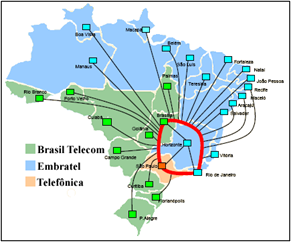
\includegraphics[width=.6\textwidth]{img/exemplo-conexoes.png}
    \legend{Fonte: \citeonline{rappaport09}}
\end{figure}

Se a figura que for incluída se tratar de um diagrama, um gráfico ou uma ilustração de autoria própria, priorize o uso de imagens vetoriais no formato PDF. Com isso, o tamanho do arquivo final do trabalho será menor, e as imagens terão uma apresentação melhor, principalmente quando impressas, uma vez que imagens vetoriais são perfeitamente escaláveis para qualquer dimensão. Veja o próprio logo do PPGEE, presente na capa e na folha de rosto, que está no formato PDF, bem como a \autoref{fig:exemplo-mlp}. Se for utilizar o Microsoft Excel para produzir gráficos, ou o Microsoft Word para produzir ilustrações, exporte-os como PDF e os incorpore ao documento.

\begin{figure}[htbp]
    \centering
    \caption{\label{fig:exemplo-mlp} Rede neural \textit{perceptron} de arquitetura 2-NH-1.}
    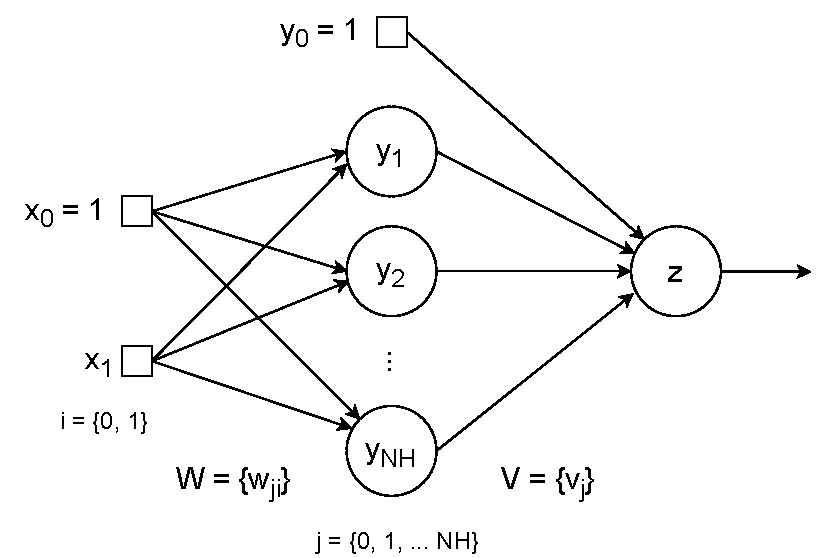
\includegraphics[width=.6\textwidth]{img/exemplo-mlp.pdf}
    \legend{Fonte: autoria própria.}
\end{figure}

Veja também a ferramenta Inkscape (\url{http://inkscape.org/}). Ela é uma excelente opção de código-livre para produzir ilustrações vetoriais, similar ao CorelDraw ou ao Adobe Illustrator. Para produzir diagramas, há também a ferramenta online \url{https://www.diagrams.net/}, que também permite a exportação direto para o formato PDF. O diagrama da \autoref{fig:exemplo-mlp} foi feito utilizando esta ferramenta.

De todo modo, caso não seja possível utilizar arquivos de imagens como PDF, pode-se utilizar qualquer outro formato, como JPEG (preferencialmente para fotos), PNG (preferencialmente para texto, diagramas ou desenhos simples) etc.

O \LaTeX{} também permite inserir subfiguras. Veja o exemplo da \autoref{fig:exemplo-subfiguras}. Pode-se também referenciar as subfiguras individualmente (\autoref{fig:subfig1} e \autoref{fig:subfig2}).

\begin{figure}[htbp]
    \centering
    \caption{\label{fig:exemplo-subfiguras} Exemplo de subfiguras.}
    \begin{subfigure}[b]{0.45\textwidth}  % tamanho da subfigura
        \centering
        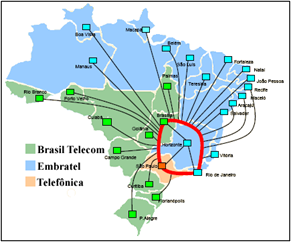
\includegraphics[width=\textwidth]{img/exemplo-conexoes.png}
        \caption{\label{fig:subfig1} subfigura à esquerda}
    \end{subfigure}
    \hfill
    \begin{subfigure}[b]{0.5\textwidth}  % tamanho da subfigura
        \centering
        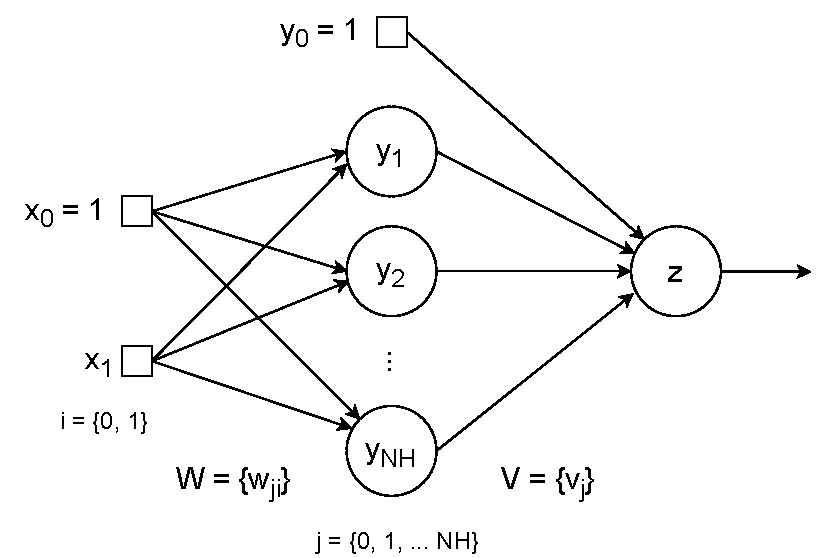
\includegraphics[width=\textwidth]{img/exemplo-mlp.pdf}
        \caption{\label{fig:subfig2} subfigura à direita}
    \end{subfigure}
\end{figure}

\subsection{Exemplo do Uso de Tabelas}

Em tabelas deve-se evitar o uso de bordas verticais para separar as colunas e bordas horizontais para separar as linhas. Somente o cabeçalho pode apresentar bordas horizontais para separar os títulos das colunas. Ao final da tabela é utilizada uma borda horizontal. Veja o exemplo da \autoref{tab:exemplo}.

\begin{table}[htb]
    \centering
    \caption{\label{tab:exemplo} Atividades desenvolvidas.}
    \begin{tabular}{ll}
        \toprule
        PERÍODO & ATIVIDADE \\
        \midrule
        EM 2006 (DEZ) & - Treinamento\\
        EM 2008 (JAN/FEV/MAR) & - Atividades de Gerenciamento de Redes\\
        & - Manutenção da Rede Física de Dados e Voz Local\\
        \bottomrule
    \end{tabular}
\end{table}

Pode-se utilizar a ferramenta online \url{https://www.tablesgenerator.com/} para elaborar tabelas \LaTeX{} de forma visual. Mude a opção ``\textit{Default table style}'' para ``\textit{Booktabs table style}'' (não precisa incluir o pacote \texttt{booktabs}, a classe \texttt{ppgee} já inclui este pacote).

\subsection{Exemplo do Uso de Alíneas}

Quando for necessário enumerar diversos assuntos de uma seção que não possua título, esta deve ser subdividida em alíneas. As alíneas, segundo a ABNT NBR 6024, devem ser apresentadas da seguinte forma:

\begin{alineas}
    \item Primeira Alínea:
    \begin{subalineas}
        \item Outros dados adicionais.
    \end{subalineas}
    
    \item Segunda Alínea:
    \begin{subalineas}
        \item Dados adicionais.
    \end{subalineas}
\end{alineas}


\subsection{Citação no Texto}

As citações devem ser indicadas no texto por um sistema de chamada: numérico ou autor-data \cite{NBR6023}. A seleção do sistema de chamada é feita no cabeçalho do arquivo \LaTeX, como opção do pacote \texttt{abntex2cite}. Para usar o sistema numérico, use a opção \verb|[num]|, ou para usar o sistema autor-data, use a opção \verb|[alf]|.

\begin{verbatim}
\usepackage[num]{abntex2cite}  % sistema numérico; ou
\usepackage[alf]{abntex2cite}  % sistema autor-data
\end{verbatim}

As citações podem ser diretas (somente no sistema autor-data): ``De acordo com \citeonline{engelbrecht2007}...''; ou indiretas \cite{engelbrecht2007}. Consulte o manual do pacote \texttt{abntex2cite} \cite{abntex2cite} para mais informações sobre o sistema numérico, ou o documento suplementar \texttt{abntex2cite-alf} \cite{abntex2cite-alf} para mais informações sobre o sistema autor-data.

A ABNT NBR 10520:2002, seção 5.3, descreve que citações diretas com mais de três linhas devem ser destacadas com recuo de 4 cm da margem esquerda, com letra menor que a do texto utilizado e sem as aspas. Para inserir citações longas, utilize o ambiente \texttt{citacao}, conforme o exemplo:

\begin{citacao}
As citações diretas, no texto, com mais de três linhas, devem ser destacadas com recuo de 4 cm da margem esquerda, com letra menor que a do texto utilizado e sem as aspas. No caso de documentos datilografados, deve-se observar apenas o recuo \cite[5.3]{NBR10520}
\end{citacao}

O ambiente \texttt{citacao\oarg{language}} pode receber como parâmetro opcional um nome de idioma previamente carregado nas opções da classe. Nesse caso, o texto da citação é automaticamente escrito em itálico e a hifenização é ajustada para o idioma selecionado na opção do ambiente, conforme o exemplo:

\begin{citacao}[english]
But what is intelligence? Dictionaries define intelligence as the ability to comprehend, to understand and profit from experience, to interpret intelligence, having the capacity for thought and reason (especially to a high degree). Other keywords that describe aspects of intelligence include creativity, skill, consciousness, emotion and intuition. \cite{engelbrecht2007}
\end{citacao}


\include{textual/metodologia}
\include{textual/resultados}
\chapter{Conclusão}

Parte final do texto, na qual se apresentam conclusões correspondentes aos objetivos ou hipóteses. NOTA: É opcional apresentar os desdobramentos relativos à importância, síntese, projeção, repercussão, encaminhamento e outros. 



% ----------------------------------------------------------
% ELEMENTOS PÓS-TEXTUAIS
% ----------------------------------------------------------
\postextual

% ----------------------------------------------------------
% Referências bibliográficas
% ----------------------------------------------------------
\bibliography{referencias}
% ---


\apendices

\chapter{Texto de autoria própria}

Elemento opcional, o apêndice é um texto ou documento de \textbf{autoria própria}, a fim de complementar sua argumentação, sem prejuízo da unidade nuclear do trabalho. O(s) apêndice(s) é(são) identificado(s) por letras maiúsculas consecutivas, travessão e pelos respectivos títulos.

\begin{anexosenv}
\chapter{Texto de terceiros}

Elemento opcional, que consiste em um texto ou documento que \textbf{não é de autoria própria}, que serve de fundamentação, comprovação e ilustração. O(s) anexo(s) é (são) identificado(s) por letras maiúsculas consecutivas, travessão e pelos respectivos títulos.

\end{anexosenv}

\end{document}
